\chapter{Introduction}
\section{Why interpretability?}
Modern machine learning models based on deep neural networks are achieving remarkable performance in many fields. In comparison with classic machine learning technologies like decision trees, it is much harder to explain how these neural networks came to their conclusions, because they use thousands to millions of training parameters.

Especially in the medical imaging field, it is very important that algorithms not only generate a correct diagnosis when training the algorithm, but also shows that its using the same cues in images as do trained physicians. These cues are found and verified in scientific studies, and therefore are well understood and proved to be correct. A wrong diagnosis generated by a neural network reduce the confidence of physicans using the technology or can even be life threatening when used without professional supervision.

\section{Image classification}
In recent years, many methods for the interpretability of deep (convolutional) neural networks have been proposed, e.g. LIME \cite{ribeiro2016should}, RISE \cite{Petsiuk2018rise}, Grad-CAM \cite{selvaraju2017grad} or DeepLIFT \cite{shrikumar2017learning}.

\begin{figure}[h]
\centering
\caption{Examples of some interpretability methods for image classification \cite{visualattribution}}
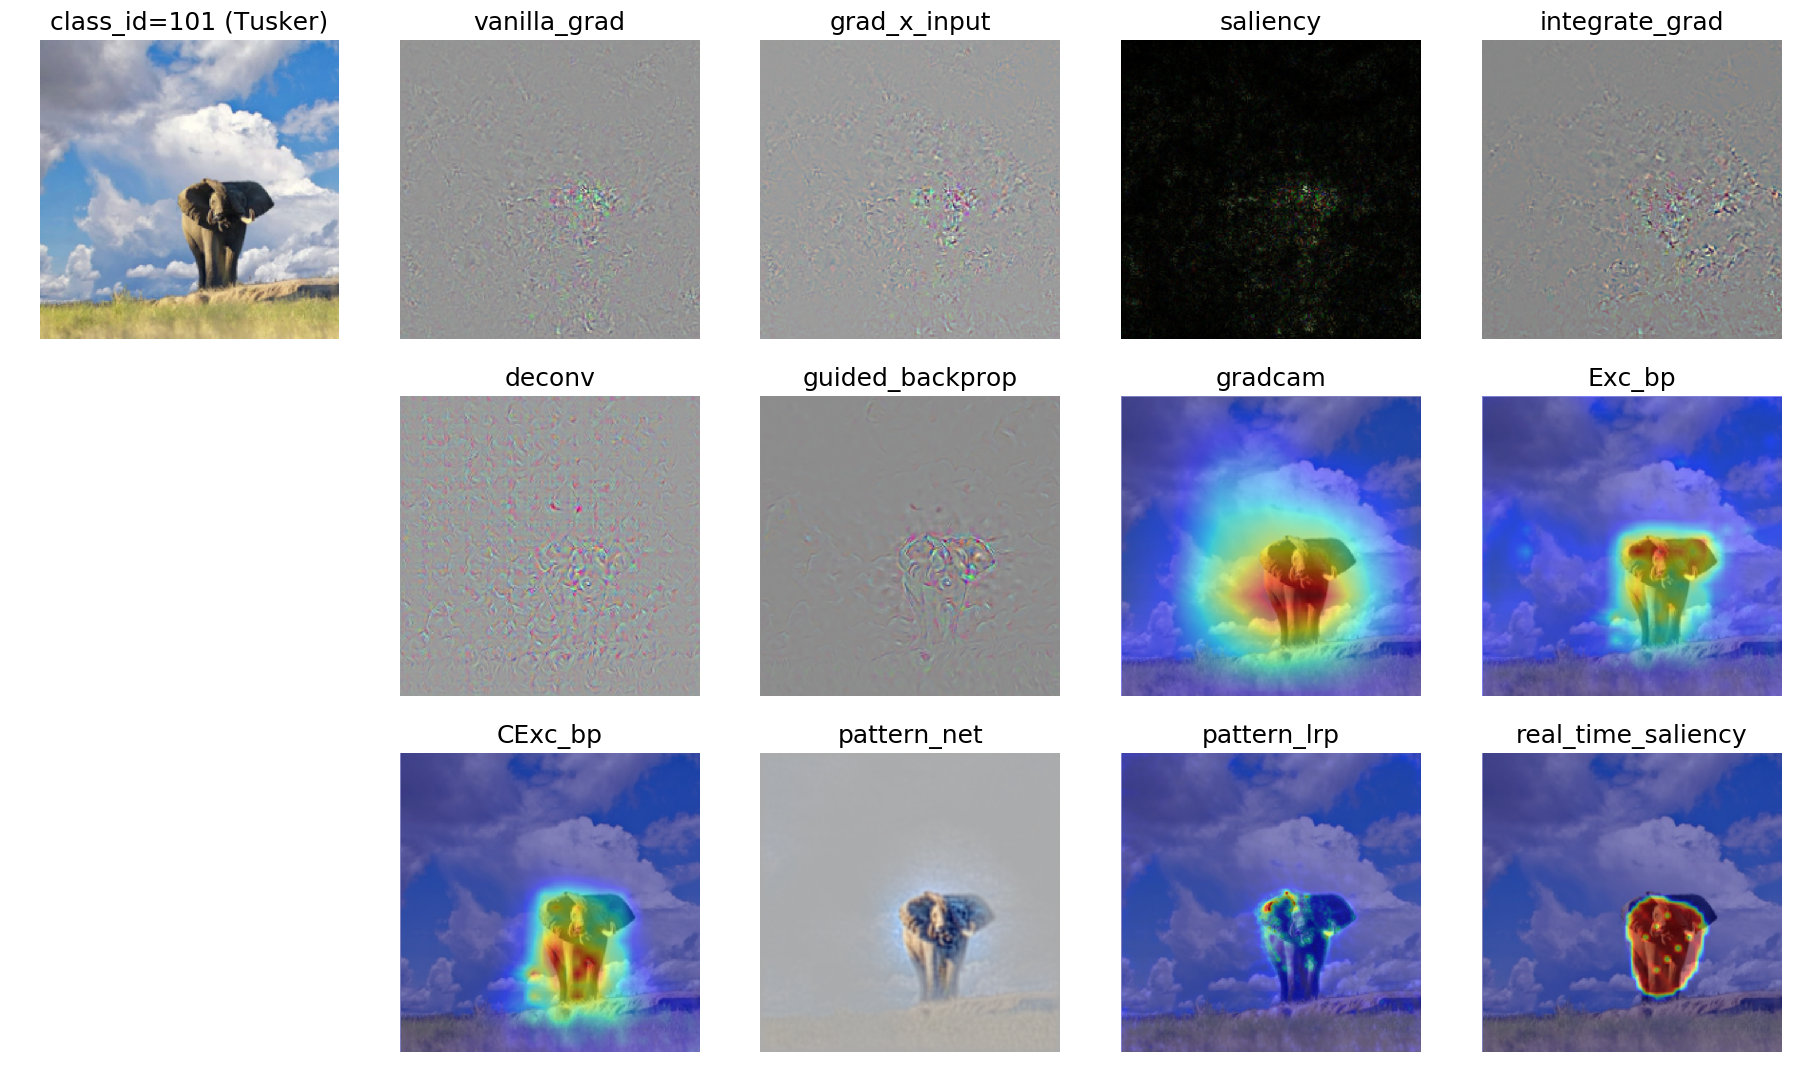
\includegraphics[width=14cm]{images/tusker_saliency.png}
\end{figure}

These methods focus on providing explanations and interpretability of classification problems for datasets like ImageNet \cite{imagenet_cvpr09} or MNIST \cite{lecun-mnisthandwrittendigit-2010}. Classification means that an algorithm can tell what is displayed on an image, e.g. if and what kind of disease is visible on a x-ray or MRI scan.

\section{Image segmentation}
Image segmentation is different from classification in the way that the algoriths do not detect what is visible on a picture, but instead mark a region (the segment) in an image where it thinks something is visible. For example for self driving cars, it is important to know where the car or pedestrian in front of the car is. 

In the medical imaging field, one applications is the segmentation of tumors in MRI scans.

\section{Interpretability on image segmentation}
TODO => does not really exist yet

\section{Source Code}
The source code of the thesis is available on GitHub:
\begin{itemize}
    \item Thesis source code (mostly jupyter notebooks): \url{https://github.com/andef4/thesis-code}
    \item Python library source code: \url{https://github.com/andef4/interpret-segmentation}
    \item Latex source for this document: \url{https://github.com/andef4/interpret-segmentation}
\end{itemize}

All source code is licensed under the permissive MIT license.

\chapter{Interpretability methods}
\section{Whitebox and blackbox methods}
One of the main questions we have to answer is which methods for interpretability can be used on an Image Segmentation task.
Generally there are two types of methods for interpretability: Blackbox and whitebox. Blackbox methods like LIME or RISE do not need insight into the underlying model and can therefore be used on arbitrary network architectures and even non-deep learning technologies like decision trees.

Whitebox methods need to have access to the underling model (e.g. weights and activation values in a neural network), because they analyze a certain part of the network.

\section{Methods overview}

https://medium.com/@keremturgutlu/semantic-segmentation-u-net-part-1-d8d6f6005066


\begin{tabular}{| p{7cm} | p{2.5cm} | p{6cm} | }
\hline
\textbf{Method} & \textbf{Model blackbox} & \textbf{Works with PyTorch} \\ \hline
RISE\cite{Petsiuk2018rise} & Yes & Supported out of the box \\ \hline
LIME\cite{ribeiro2016should} & Yes & Library independent \\ \hline
Layer-wise Relevance Propagation (LRP) & No & Should be possible  https://github.com/Hey1Li/Salient-Relevance-Propagation missing batch norm \\ \hline
DeepLIFT & No & Initial implementation in SHAP\cite{NIPS2017_7062} \\ \hline
Prediction Difference Analysis \cite{todo} & ? & ? \\ \hline
PatternNet & ? & ? \\ \hline
Deep Taylor & ? & ? \\ \hline
Grad-CAM (Selvaraju 2017) & No & Many implementations \\ \hline
SHAP DeepExplainer\cite{NIPS2017_7062} & ? & ? \\ \hline
SHAP KernelExplainer\cite{NIPS2017_7062} & ? & ? \\ \hline
Meaningful Perturbation (Fong 2017)\cite{todo} & Yes & Implementation exitst \cite{todo} https://github.com/jacobgil/pytorch-explain-black-box \\ \hline
Excitation Backprop (Zhang 2016)\cite{todo}  & ? & ? \\ \hline
\end{tabular}

% many implementations: https://github.com/yulongwang12/visual-attribution

fong has many references

% https://github.com/marcoancona/DeepExplain/blob/master/docs/comparison.png
good images: fong 2017

Baehrens'10 Gradient
Sundarajan'17 Int Grad
Zhou'16 GAP
Haufe'15 Pattern
Symonian'13 Gradient
Zeiler'14 Occlusions
Zurada'94 Gradient
Poulin'06 Additive
Zeiler'14 Deconv
Landecker'13 Contrib Prop
Caruana'15 Fitted Additive
Bazen'13 Taylor
Springenberg'14 Guided BP


%Zintgraf'17 Pred Diff  https://arxiv.org/pdf/1702.04595.pdf
%Ribeiro'16 LIME
% Fong'17 M Perturb
% Lundberg'17 Shapley
%Montavon'17 Deep Taylor
%Bach'15 LRP
%Kindernnans'17 PatternNet
%Shrikumar'17 DeepLIFT
%Zhang'16 Excitation Backprop
%Selvaraju'17 Grad-CAM

\section{Method selection}
\section{RISE}
Similar technology as LIME, uses PyTorch. Newer than LIME, paper asserts to be better.

Written for PyTorch

\section{LIME}
\section{Grad-CAM}











\chapter{Classification}
\chapter{NIH Chest X-ray}
To find out what outputs the different methods generate, we started with a simple classification task in the medical image field:

\section{Model Training}
\subsection{Inception Resnet v2}
\begin{itemize}
    \item  chest x-ray, sample data set (small subset)
    \item  multi label classification
    \item  current state of the art networkj: inception  resetnet v2 (accurate + fast to train on single GPU) \cite{todo}
    \item  using learnings and code from project2
    \item  slightly modified inception resnet v2 implementation (grayscale instead of color)
    \item  did not work, convert to RGB and downscale images (offline, preprocess.ipynb)
    \item  results: 40\% validation accuracy => bad
    \item smaller batch size (citation needed) 5, => not better
    \item next: use full dataset
    \item download 42 gigs of data
    \item simple python multiprocessing for preprocessing
\end{itemize}

\subsection{ResNet}
Instead of waiting for the expected very long learning time for Inception-Resnet V2, we did a short test with Resnet50 with pretrained parameters (ImageNet) on the sample dataset. Only the last layer is unfreezed.

\begin{itemize}
    \item Epoch time of ~40 seconds instead of (TODO) 10 minutes/3 hours for full dataset
    \item resnet50 with pretrained
    \item resnet50 without pretrained
    \item resnet18 without pretrained
    \item resnet18 without pretrained full dataset
\end{itemize}

\subsection{Only images with actual diagnosis}
https://www.kaggle.com/kmader/train-simple-xray-cnn 
For testing out the methods, images with findings are much more helpful, so filter them out.

Better results:


\subsection{Single label only}
65\%

\subsection{Densenet}
% https://medium.com/@jrzech/reproducing-chexnet-with-pytorch-695ff9c3bf66

Loading the saved model did not work, because the used version of PyTorch was old and incompatible with ours.

=> Retraining

\subsubsection{Image resize problems}
In the Densenet code there was a reference that some images were not properly resized. We did a short check on our preprocessed data, but it revelead no such problems. Used bash command:

\begin{minted}{bash}
find . -name '*.png' -exec file {} \; | cut -c 37-45 | uniq
\end{minted}

\subsection{Densenet single}
\begin{itemize}
    \item Fail: Not correctly setting up classes (last layer has 1000 classes for imagenet, we have 14)
    \item Fail 2: Train and validation set do not have same classes because of ordering in dataset loading code
\end{itemize}

After training for a short time with the fixes, we get an acceptable accuracy rate of 55\%. We then started to calculate the accuracy per class, as has been done on the reproduce-chexnet discussed above. We quickly discovered that only the "No findings" class was accurate, an all other classes had zero correct classifications.

\begin{itemize}
    \item test with no findings removed => not that better, finds only 3 classes correctly
    \item try with weighted cross entropy loss
\end{itemize}


\section{Methods}

\subsection{RISE}
Problem: returned classes from RISE do not match with precalculated classes
=> normalize was not applied on find\_best\_images.
=> use same function on all image loaders

\subsection{LIME}
\subsection{Grad-CAM}


\chapter{Segmentation}
The scans in the BraTS 2018 datasets are created with four different settings of the MRI scanner:

\begin{itemize}
    \item Native (T1)
    \item Post-contrast T1-weighted (T1Gd)
    \item T2-weighted (T2)
    \item T2 Fluid Attenuated Inversion Recovery (FLAIR)
\end{itemize}

Every layer is saved as a 2 byte signed integer. We convert these to 1 byte unsigned integers and scale the range to 0-255, so the highest value in the 2 byte signed integer is 255 and the lowest is 0.
This way we generate a grayscale image that can be viewed with a normal image viewer and should be processable by a normal convolutional neural network

\section{Segments}
The scanners detect three different types of kinds of tumor tissues. These are also saved as 2 byte integers with the values 0 (not tumor), 1 (todo), 2(todo) and 4(todo).


GD-enhancing tumor (ET — label 4),
peritumoral edema (ED — label 2),
necrotic and non-enhancing tumor core (NCR/NET — label 1)

% https://www.researchgate.net/post/What_are_the_differences_between_enhancing_and_nonenhancing_lesions_in_MRI


Gadolinium is a chemical compound given during MRI scans that highlights areas of inflammation (Active Lesions). A gadolinium-enhanced  MRI scan shows active lesions, meaning that there is a breakdown of the blood-brain barrier and inflammation is present.


\section{Train}
https://github.com/milesial/Pytorch-UNet
https://github.com/usuyama/pytorch-unet

modifications: do not use deprectated functions

first try. baaad
second try with normalization: no change
build evaluation
third try with batch norm: much higher loss that slowy goes down, evaluate still shows random pixels
5. run it for some hours, it worked!

\chapter{Testnet}
\section{Introduction \& Motivation}
\section{Applying RISE}
\section{Applying Grad-CAM}

\chapter{Modified BraTS with tumor contours}
\section{Introduction \& Motivation}
\section{Applying RISE}

\chapter{Hausdorf Distance masks}
\section{Introduction}
\section{Hausdorff distance}
\section{Masking}
\section{Visualization}
\section{Applying HDM on Testnet}
\section{Applying HDM on BraTS}
\section{Applying HDM on modified BraTS}
\section{Applying HDM on BraTS 3D}

\chapter{Infrastructure \& tooling}
\section{Infrastructure setup}
Computer reachable from internet, running jupyter with password,
rtx 2080

\section{Scripts}

\section{Testing}


\chapter{Discussion}
compare with requirements document

\chapter{Conclusion}